\section*{Methodology}

The intention of this work is to create a mobile robot that can plan its movements without any map knowledge on the environment. Its translation function is defined as:
\begin{equation}
v_t = f(x_t, p_t, v_{t-1})
\end{equation}
where $x_t$ is the observation from the raw sensor information, $p_t$ is the relative position of the target, and $v_{t-1}$ is the velocity of the mobile robot in the last time step.
All variables specified, previously, can be defined as the current state $s_t$ of the mobile robot.
With this model it is possible to get the actions that the robot will make, given its current state.
However, it is needed to ensure a minimum reading frequency of the input data to control the movement of the robot because if the robot get a slow read frequency of the inputs it cannot react to an obstacle in the trajectory to a target. In this way, the robot can react to new states quickly.
This methods was first explored by Tai \textit{et al.} \cite{tai2017virtual}.

\subsection*{Network Structure}

Once the system of state and actions has been defined, it is possible to create a DDPG network capable of resolving the problem.
The DDPG network has 14 inputs as presented in Fig. \ref{fig:entradaESaida}, in which 10 corresponds to the laser range findings, 2 corresponds to the linear and angular velocity, and the other 2 corresponds to the relative position and angle of the mobile robot to the target.
The sample of the laser range findings are between $-90$ and $90$ degrees in relation to the robot. The output of the network is the action of linear and angular velocity that will be applied on the mobile robot.

\begin{figure}
\centerline{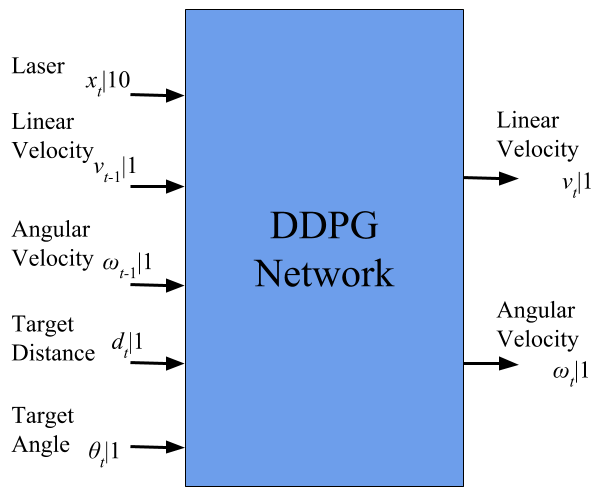
\includegraphics[width=\columnwidth]{images/o_and_i.png}}
\caption{DDPG network inputs and outputs.}
\label{fig:entradaESaida}
\end{figure}

The network structure of the DDPG is shown in Fig \ref{fig:projetointegrador}. 
The actor-network has as input the current state of the mobile robot followed by 3 fully-connected neural networks layers with 512 nodes.
This input of the networks is transformed on the linear and angular velocity that will be the commands sent to the motor of the mobile robot. 
The angular velocity range is constrained between $(-1,1)$ and the hyperbolic tangent function $(tanh)$ is used as activation function.
For the linear angular range, that it is constrained between $(0,1)$, the sigmoid function was used.
As there is no laser readings in the back of robot, the backward move is not necessary.
The output actions are then multiplied with two hyperparameters to decide the final linear and angular velocity executed by the mobile robot.
For this, it was used as maximum linear velocity $0.22$ $m/s$ and maximum angular velocity $1$ $rad/s$ on the TurtleBot3 robot version Burger.


\begin{figure}
\centerline{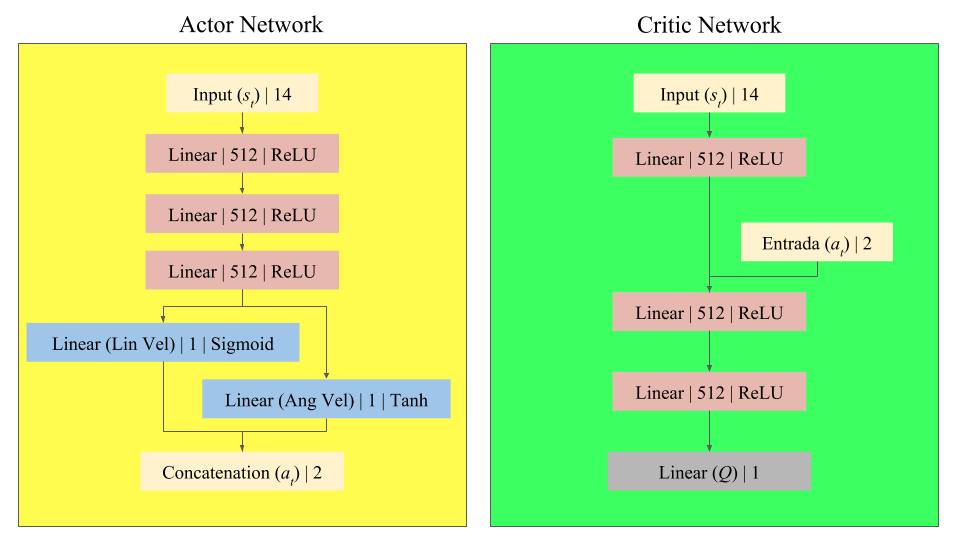
\includegraphics[width=\columnwidth]{images/projeto_integrador_en.png}}
\caption{DDPG network structure model.}
\label{fig:projetointegrador}
\end{figure}

In the critic-network, the Q-value of the current state and action are predicted.
Using only 3 fully-connected neural networks layers to process the input state.
Where the action, output of the actor-networks, is concatenated on the second neural network layer.
The Q-value is activated through a linear activation function:
\begin{equation}
y = kx +b
\end{equation}
where $x$ is the input of the last layer, $y$ is the predicted Q-value, and $k$ and $b$ are the trained weights and bias of this layer, respectively.

\subsection*{Simulation Environments}

There were used three environments for the simulations. The first environment is  shown in Fig. \ref{fig:environments}(a), the environment represents a free area for the robot to move.
The walls of this environment are the only things where the robot can collide.
If the mobile robot collide with the wall or any obstacle, a negative reward is given for this action and the current episode stops.

\begin{figure}
\centerline{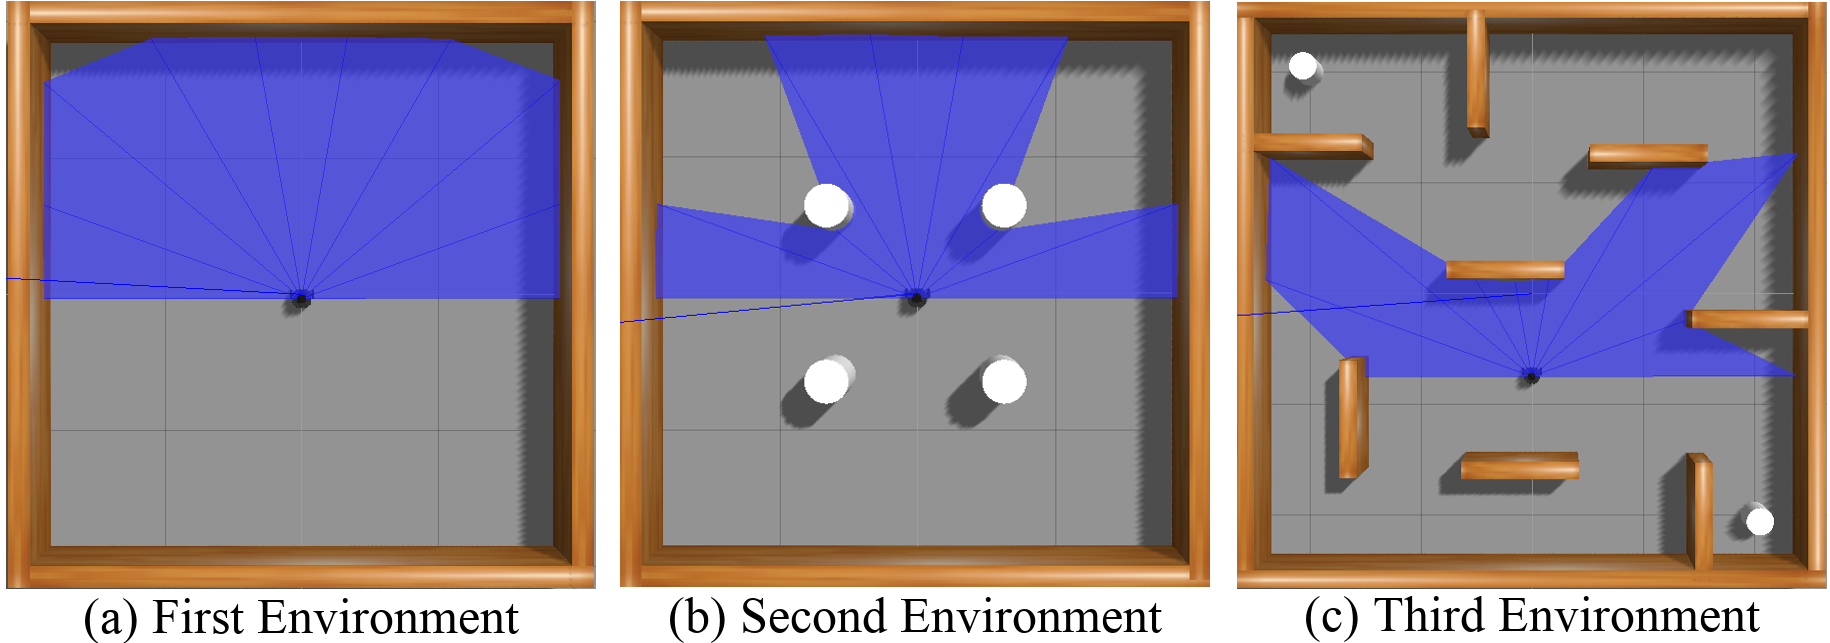
\includegraphics[width=\columnwidth]{images/environments1.png}}
\caption{Training environments used on Gazebo simulation.}
\label{fig:environments}
\end{figure}

The second environment is shown in Fig. \ref{fig:environments}(b) and has 4 fixed obstacles.
It means that this environment is more complex in a way that the intelligent agent have to make a better strategy to not collide.

The third environment, shown in Fig. \ref{fig:environments}(c), is more complex than the previous environments.  
The number of walls and the mobile obstacles, represented by the white blocks, makes the environment more dynamical, approaching it to a real-world environment.

\subsection*{Reward Function}

Once the environment have been defined it is possible to simulate a controlled mobile robot for a navigation task.
Now it is necessary to define the reward and penalty system to the Deep-RL network.
Remembering that the rewards and penalties are attributed numbers passed to the intelligent agent.
So, the network will make a feedforward and backpropation step in order to learn the hyperparameters.

There are four different conditions for the reward system that presented better results for the problem's resolution and are the following:
\begin{equation}
r (s_t, a_t) = 
\begin{cases}
r_{arrive} \ \textrm{if} \ d_t < c_d
\\
r_{collide} \ \textrm{if}\ min_x < c_o
\\
c_{r1}(d_{t-1} - d_t) \ \textrm{if} \ (d_{t-1} - d_t) > 0
\\
c_{r2} \ \textrm{if} \ (d_{t-1} - d_t) \leq 0
\end{cases}
\end{equation}

If the robot gets to the target through threshold checking $c_d$, a positive reward $(r_{arrive})$ is given, but if the robot collides with an obstacle through a minimum range readings checking, a negative reward $(r_{collide})$ is given.
Both conditions are sufficient to end the training episode.
Otherwise, the reward is based on the distance difference from the target compared to the last time step $(d_{t-1} - d_t)$. 
If this difference is positive the reward given is the distance traveled multiplied by the hyperparameter $(c_{r1})$, and if the distance is negative is used the hyperparameter $(c_{r2})$.
This motivates the mobile robot to get closer to the target position and encourages it to avoid the obstacles in the environment.


